\documentclass{article}
\usepackage{hyperref}
\usepackage{amsmath}
\usepackage{amssymb}
\usepackage{pgfplots}
\usepackage{float}
\usepackage{todonotes}
\usepackage{tikz}
\usepackage[shortlabels]{enumitem}

\renewcommand{\Re}{\mathbb{R}}
\newcommand{\Li}{\mathcal{L}}
\newcommand{\Ex}{\mathbb{E}}
\renewcommand{\Pr}{\mathbb{P}}
\newcommand{\Hy}{\mathcal{H}}
\newcommand{\sign}{\text{sign}}
\newcommand{\error}{\text{error}}

\newcommand\bigO[1]{
    \ensuremath{\mathcal{O}\left(#1\right)}
    }

\newcommand{\sigmoidPlot}{
    
    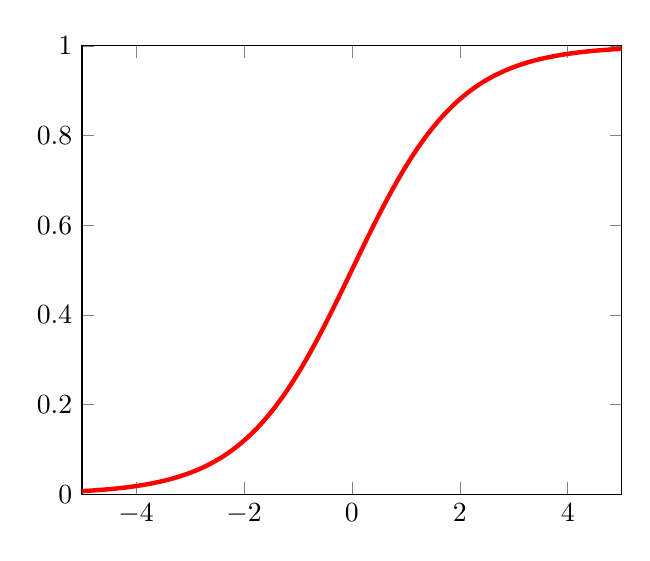
\begin{tikzpicture}
        \begin{axis}[xmin=-5, xmax=5, ymin=0, ymax=1, samples=150]
        \addplot[red, ultra thick] {1/(1+exp(-x))};
        \end{axis}
    \end{tikzpicture}
    
    }

\usetikzlibrary{positioning, calc}
\usetikzlibrary{arrows.meta}

\tikzstyle{circlebox}=[circle,thick,draw=black!75,minimum size=8mm]
\tikzstyle{inputnode}=[circlebox, draw=blue!75]
\tikzstyle{hiddennode}=[circlebox, draw=orange!75]
\tikzstyle{outputnode}=[circlebox, draw=orange!75]
\tikzstyle{simplebox}=[rectangle,thick,draw=black!75,
fill=black!20,minimum size=4mm]
\tikzstyle{textbox}=[rectangle,thick,minimum size=4mm,draw=black!0,
fill=black!0]
\tikzstyle{halfvdistance}=[yshift=-0.7cm]
\tikzstyle{abovebetween}=[xshift=-2.7mm]
\tikzstyle{edgepath} = [-Latex,->,shorten >=1pt,-stealth,semithick, rounded 
corners=5pt]

\def \nodedv {0.735cm}
\def \nodedh {0.65cm}

\tikzset{
    between/.style args={#1 and #2}{
        at = ($(#1)!0.5!(#2)$)
    }
}

\begin{document}
    \section{Subjects}
    \begin{itemize}
        \item Different distance measures between evolutionary trees
        \item Computing distance between trees
    \end{itemize}
    
    \section{Notes}
    
    \subsection{Phylogenetic trees}
    There is strong evidence that all life on earth is decended from a single 
    common ancestor. Over the course of at least 3.8 billion years, that life 
    form has changed and split itself into new and independent lineages. The 
    evolutionary relationships among these species is referred to as their 
    phylogeny, phylogenetic reconstruction is concerned with inferring the 
    phylogeny of groups of organisms.
    
    We call these groups \textit{taxa} (or singular taxon), the splitting of 
    lineages is called \textit{speciation} (think of splitting it into 
    different species). Usually speciation happens if one population is split 
    into two that can no longer interbreed (e.g. if a river splits them apart). 
    We can use methods of phylogenetic to contemplate over the tree of life, or 
    simply to inferr the phylogeny of different populations within a species.
    
    In a rooted phylogenetic tree $T$, the root node $r$ corresponds to the 
    last common ancestor of all species in $T$, we then call a path from the 
    root to a leaf an \textit{evolutionary path}. If an equal amount of change 
    occurs on every evolutionary path (i.e. each species have the same amount 
    of ``change'') then the evolutionary change occur in a more-or-less 
    clocklike fashion and we then say that this tree satisfies the 
    \textit{molecular clock hypothesis}, we can then assign a time $t(v)$ to 
    every internal node $v$ in the tree and a length of $t(v)-t(w)$ to an edge 
    $(v,w)$ in the tree.
    
    Every extant (still alive) species corresponds to time $0$, and a 
    speciation event (internal node $v$) occured in the tree $t(v)$ time ago. 
    We then have that the length of an edge represents the amount of time that 
    lies between two speciation events.
    
    Furthermore, the last common ancestor (root) lived $t(r)$ and all 
    evolutionary paths have the same length $t(r)$ where the length of a path 
    is the sum of the lengths of all edges along the path.
    
    Once the \textit{molecular clock hypotheses} was widely accepted, but has 
    since been disproven so now time instead refers to the expected amount of 
    evolution.
    
    \subsubsection{Distance methods}
    Distance methods construct a phylogenetic tree from a distance matrix that 
    contains the evolutionary distances between all pairs of taxa (groups of 
    organisms). If we ignore edge weights, we speak of the topology (shape) of 
    a tree, and it turns out that we have methods that \textit{provably} find 
    the correct tree if the distance matrix is ultrametric, and some that works 
    if the distance matrix is additive. However the data we can record is 
    usually approximation of the true (additive) data, and thus we can't rely 
    on the distance matrix being additive. However, it turns out that the 
    methods can still find the correct \textit{topology} of the tree under 
    certain criteria.
    
    If we just have the topology, then we must assign weights to the edges of 
    the tree that best fit the data, which can be done with the least squares 
    methods.
    
    \subsubsection{Basic definitions}
    Phylogenies are usually represented as binary trees, because generially 
    speciation happens when one lineage splits into two independent lineages. 
    This is not entirely correct, sometimes horizontal gene-transfer happens 
    and hybrid speciation but it is rare. So for simplicity we just look deal 
    with phylogenetic trees, however let's not insist they have to be binary 
    for the moment:
    
    Let $S=\{s_1,\dots,s_n\}$ be a set of taxa. A phylogenetic tree on $S$ is a 
    triple $T=(V,E,\alpha)$ where:
    \begin{itemize}
        \item $V$ is the set of nodes, $E$ is the set of undirected edges
        \item $(V,E)$ is a an acyclic connected graph, in which there might be 
        a distinguished root node of degree $\geq 2$ and all other internal 
        nodes have a degree $\geq 3$. So either rooted or unrooted. We will 
        denote the set of leaves by $V_L$ and the set of internal nodes by $V_I$
        \item $\alpha$ is a bijection $\alpha: S \rightarrow V_L$ between the 
        set of taxa and the set of leaves
    \end{itemize}
    An edge $(v,w) \in E$ is an external edge if either $v$ or $w$ is a leaf. 
    Otherwise it is an internal edge.
    
    We haven't included edge-weights here, they will be introduced later.
    
    \subsection{Distance between tree-topologies}
    Distance between trees is about measuring how far they are from each other, 
    that is, how different are they. There are a number of different ways that 
    have been proposed to this end, we will start by looking at the measures 
    that compute the distance between the topologies of trees.
    
    \subsubsection{The symmetric difference}
    If we ignore the edge weights, then each edge can be seen as a branch which 
    divides the species into a partition with two sets. If we make a list of 
    the partitions each tree implies (e.g. $AB|CD$ and $A|B$ and $C|D$)  we 
    will then simply count how many partitions are in one list which is not in 
    the other and that will be the symmetric difference.
    
    The symmetric distance is very easy to compute, but is very sensitive to 
    all differences between trees. Therefore a tree which has partial 
    similarities, might still score the maximum possible distance.
    
    This can also be named the Robinson-Fould distance
    
    \subsubsection{The quartets distance}
    The \textit{quartets distance} is more sensitive to partial similarities of 
    structures between trees. A quartet is four named species in an unrooted 
    tree. Quartet topology is the topology of the quartet induced by the tree. 
    
    The quartet distance is then simply the number of quartets that don't have 
    the same topology in the two trees. Computing this distance can be done in 
    \bigO{n^2}. It has been shown that it can be done in \bigO{n(\ln n)^2}
    
    \subsubsection{Nearest-Neighbour interchange distance}
    Simply, compute the minimum number of nearest-neighbour interchange 
    re-arrangements that are needed to go from one tree to the other. Does not 
    have teh same issue with tree-distance symmetric distance, however it is 
    NP-Complete.
    
    \subsubsection{Computing RF-Distance}
    There are various ways to compute the Robinson Fouls distance (also called 
    the symmetric difference). The \bigO{n} algorithm proposed by Day. So here 
    come's Day's algorithm for computing the RF-Distance:
    \begin{itemize}
        \item Root both trees by the same leaf
        \item Do a DFS numbering of $T_1$
        \item Assign the same numbers to $T_2$
        \item Find all the ``valid'' intervals in $T_1$ and $T_2$
        \item Count the number of intervals that don't exist in both $T_1$ and 
        $T_2$
    \end{itemize}
    
    \subsection{Distance between trees}
    Now, there are some distance-measures that take the branch-weights into 
    account.
    
    The Robinson Foulds distance can be taken into account by, for each edge, 
    compute the difference of the weights. If an edge exists in one and not the 
    other (i.e. the case where we would nomrally count one up) we add the 
    complete weight of the edge.
    
    \subsubsection{Computing the Quartet distance}
    The triplet and quartet distance are very close, I will focus on the 
    Quartet distance.
    
    First let's look at some of the cases, the Quartet distance counts the 
    number of quartets where the two trees disagree. To this end there are 
    ``resolved'' and ``unresolved'' cases, the unresolved case, is when all the 
    leaves are connected through a single node (all same parent).
    
    If both $T_1$ and $T_2$ deems the quartet to be unresolved, then they agree 
    if either one or the other think it's unresolved then they disagree. If 
    they both think it's resolved then they agree if they have the same 
    topology. So we count the number of times they disagree. The number of 
    quartets is $\begin{pmatrix}
    n\\
    4
    \end{pmatrix}$.
    \\
    \\
    Let's just look at binary trees, if we are dealing with binary trees, then 
    the unresolved case is not possible, thus we just look at the quartets 
    where the topologies differ.
    
    A dynamic programming approach, conceptually we simply say that each edge 
    is oriented both ways, we then say that $F_1 \xrightarrow{e_1}(F_2, F_3)$ 
    in $T_1$, \textit{claims} all quartets, $ij|kl$ with $i,j \in F_1$ and 
    either $ k \in F_2$ and $l \in F_3$ or vice versa, where $F_1$ is the tree 
    behind the edge and $F_2, F_3$ is the two subtrees in front of the edge. 
    Every shared quartet is counted twice, so we divide by two. Giving us the 
    formula:
    
    \begin{equation*}
        Count(e_1,e_2) = \begin{pmatrix}
        |F_1 \cap G_1|\\
        2
        \end{pmatrix}
        (|F_2 \cap G_2| \cdot |F_3 \cap G_3| + |F_2 \cap G_3| \cdot |F_3 \cap 
        G_2|)
    \end{equation*}
    \begin{equation*}
        d_{quartet}=\begin{pmatrix}
        n\\
        4
        \end{pmatrix}
        - \frac{1}{2} \sum_{e_1,e_2} Count(e_1, e_2)
    \end{equation*}
    
     and then we count the how many of these edges $ij 
    \rightarrow kl$ are claimed by both trees. This can be done in \bigO{n^2}.
    
    There is another way that is based on tree coloring that can do it in 
    \bigO{n \log n}
\end{document}